\documentclass{article}\usepackage[]{graphicx}\usepackage[]{color}
%% maxwidth is the original width if it is less than linewidth
%% otherwise use linewidth (to make sure the graphics do not exceed the margin)
\makeatletter
\def\maxwidth{ %
  \ifdim\Gin@nat@width>\linewidth
    \linewidth
  \else
    \Gin@nat@width
  \fi
}
\makeatother

\definecolor{fgcolor}{rgb}{0.345, 0.345, 0.345}
\newcommand{\hlnum}[1]{\textcolor[rgb]{0.686,0.059,0.569}{#1}}%
\newcommand{\hlstr}[1]{\textcolor[rgb]{0.192,0.494,0.8}{#1}}%
\newcommand{\hlcom}[1]{\textcolor[rgb]{0.678,0.584,0.686}{\textit{#1}}}%
\newcommand{\hlopt}[1]{\textcolor[rgb]{0,0,0}{#1}}%
\newcommand{\hlstd}[1]{\textcolor[rgb]{0.345,0.345,0.345}{#1}}%
\newcommand{\hlkwa}[1]{\textcolor[rgb]{0.161,0.373,0.58}{\textbf{#1}}}%
\newcommand{\hlkwb}[1]{\textcolor[rgb]{0.69,0.353,0.396}{#1}}%
\newcommand{\hlkwc}[1]{\textcolor[rgb]{0.333,0.667,0.333}{#1}}%
\newcommand{\hlkwd}[1]{\textcolor[rgb]{0.737,0.353,0.396}{\textbf{#1}}}%

\usepackage{framed}
\makeatletter
\newenvironment{kframe}{%
 \def\at@end@of@kframe{}%
 \ifinner\ifhmode%
  \def\at@end@of@kframe{\end{minipage}}%
  \begin{minipage}{\columnwidth}%
 \fi\fi%
 \def\FrameCommand##1{\hskip\@totalleftmargin \hskip-\fboxsep
 \colorbox{shadecolor}{##1}\hskip-\fboxsep
     % There is no \\@totalrightmargin, so:
     \hskip-\linewidth \hskip-\@totalleftmargin \hskip\columnwidth}%
 \MakeFramed {\advance\hsize-\width
   \@totalleftmargin\z@ \linewidth\hsize
   \@setminipage}}%
 {\par\unskip\endMakeFramed%
 \at@end@of@kframe}
\makeatother

\definecolor{shadecolor}{rgb}{.97, .97, .97}
\definecolor{messagecolor}{rgb}{0, 0, 0}
\definecolor{warningcolor}{rgb}{1, 0, 1}
\definecolor{errorcolor}{rgb}{1, 0, 0}
\newenvironment{knitrout}{}{} % an empty environment to be redefined in TeX

\usepackage{alltt}

\usepackage{amsmath, amsthm, amsfonts}
\usepackage{enumerate}
\usepackage{hyperref}

\title{Assignment 2}
\author{Anh Le}
\IfFileExists{upquote.sty}{\usepackage{upquote}}{}
\begin{document}

\maketitle

\begin{knitrout}
\definecolor{shadecolor}{rgb}{0.969, 0.969, 0.969}\color{fgcolor}\begin{kframe}
\begin{alltt}
\hlcom{## knitr configuration: http://yihui.name/knitr/options#chunk_options}
\hlstd{opts_chunk}\hlopt{$}\hlkwd{set}\hlstd{(}\hlkwc{error}\hlstd{=} \hlnum{TRUE}\hlstd{,} \hlkwc{warning} \hlstd{=} \hlnum{FALSE}\hlstd{,} \hlkwc{message} \hlstd{=} \hlnum{FALSE}\hlstd{,}
               \hlkwc{tidy} \hlstd{=} \hlnum{FALSE}\hlstd{,} \hlkwc{cache} \hlstd{= F,} \hlkwc{echo} \hlstd{= T,}
               \hlkwc{fig.width} \hlstd{=} \hlnum{4}\hlstd{,} \hlkwc{fig.height} \hlstd{=} \hlnum{4}\hlstd{,} \hlkwc{fig.align}\hlstd{=}\hlstr{"center"}\hlstd{)}
\hlkwd{library}\hlstd{(DAAG)}
\end{alltt}


{\ttfamily\noindent\itshape\color{messagecolor}{\#\# Loading required package: lattice}}\end{kframe}
\end{knitrout}

\section{Question 1: Problem 1.2 in book}
The \verb!orings! data frame gives data on the damage that had
occurred in US space shuttle launches prior to the disastrous
Challenger launch of January 28, 1986. Only the observations in rows
1, 2, 4, 11, 13, and 18 were included in the pre-launch charts used in
deciding whether to proceed with the launch.

Create a new data frame by extracting these rows from \verb!orings!,
and plot \verb!total! incidents against \verb!temperature! for this
new data frame.  Obtain a similar plot for the full data set.

\textbf{Solution}

Use the following to extract rows that hold the data that were presented in
the pre-launch charts:
\begin{knitrout}
\definecolor{shadecolor}{rgb}{0.969, 0.969, 0.969}\color{fgcolor}\begin{kframe}
\begin{alltt}
\hlstd{orings86} \hlkwb{<-} \hlstd{orings[}\hlkwd{c}\hlstd{(}\hlnum{1}\hlstd{,}\hlnum{2}\hlstd{,}\hlnum{4}\hlstd{,}\hlnum{11}\hlstd{,}\hlnum{13}\hlstd{,}\hlnum{18}\hlstd{), ]}
\hlkwd{par}\hlstd{(}\hlkwc{mfrow}\hlstd{=}\hlkwd{c}\hlstd{(}\hlnum{1}\hlstd{,} \hlnum{2}\hlstd{))}
\hlkwd{with}\hlstd{(orings86,} \hlkwd{plot}\hlstd{(Temperature, Total))}
\hlkwd{with}\hlstd{(orings,} \hlkwd{plot}\hlstd{(Temperature, Total))}
\end{alltt}
\end{kframe}

{\centering 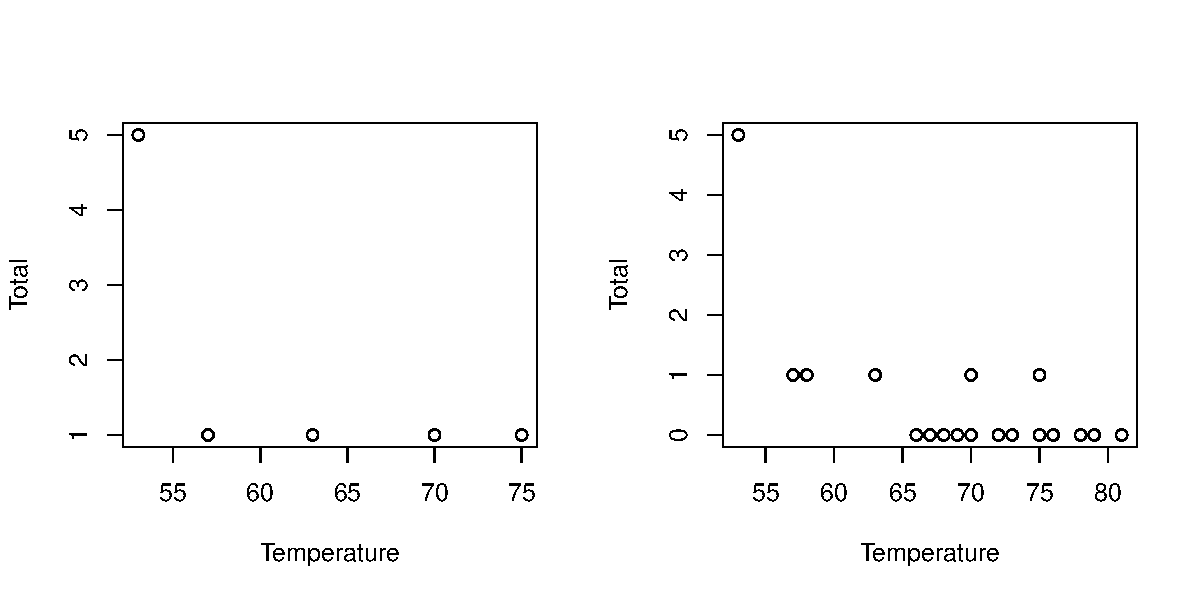
\includegraphics[width=\maxwidth]{figure/unnamed-chunk-2} 

}


\begin{kframe}\begin{alltt}
\hlkwd{par}\hlstd{(}\hlkwc{mfrow}\hlstd{=}\hlkwd{c}\hlstd{(}\hlnum{1}\hlstd{,} \hlnum{1}\hlstd{))}
\end{alltt}
\end{kframe}
\end{knitrout}

\section{Question 2: Problem 1.11 in book}

Explain the output from the final \verb!table(gender)!.

\begin{knitrout}
\definecolor{shadecolor}{rgb}{0.969, 0.969, 0.969}\color{fgcolor}\begin{kframe}
\begin{alltt}
\hlstd{gender} \hlkwb{<-} \hlkwd{factor}\hlstd{(}\hlkwd{c}\hlstd{(}\hlkwd{rep}\hlstd{(}\hlstr{"female"}\hlstd{,} \hlnum{91}\hlstd{),} \hlkwd{rep}\hlstd{(}\hlstr{"male"}\hlstd{,} \hlnum{92}\hlstd{)))}
\hlkwd{table}\hlstd{(gender)}
\end{alltt}
\begin{verbatim}
## gender
## female   male 
##     91     92
\end{verbatim}
\begin{alltt}
\hlstd{gender} \hlkwb{<-} \hlkwd{factor}\hlstd{(gender,} \hlkwc{levels}\hlstd{=}\hlkwd{c}\hlstd{(}\hlstr{"male"}\hlstd{,} \hlstr{"female"}\hlstd{))}
\end{alltt}
\end{kframe}
\end{knitrout}
\begin{knitrout}
\definecolor{shadecolor}{rgb}{0.969, 0.969, 0.969}\color{fgcolor}\begin{kframe}
\begin{alltt}
\hlkwd{table}\hlstd{(gender)}
\end{alltt}
\begin{verbatim}
## gender
##   male female 
##     92     91
\end{verbatim}
\begin{alltt}
\hlstd{gender} \hlkwb{<-} \hlkwd{factor}\hlstd{(gender,} \hlkwc{levels}\hlstd{=}\hlkwd{c}\hlstd{(}\hlstr{"Male"}\hlstd{,} \hlstr{"female"}\hlstd{))}
\hlkwd{table}\hlstd{(gender)}
\end{alltt}
\begin{verbatim}
## gender
##   Male female 
##      0     91
\end{verbatim}
\begin{alltt}
\hlkwd{rm}\hlstd{(gender)}                  \hlcom{# Remove gender}
\end{alltt}
\end{kframe}
\end{knitrout}

\textbf{Solution}

Notice that before the final \verb`table(gender)`, we make a typo, specifying \verb`levels=c("Male", "female")` instead of \verb`levels=c("male", "female")`. Since there is no \verb`"Male"` in \verb`gender`, R correctly says that there is 0 \verb`"Male"`.

The moral of this problem is that you should avoid specifying the \verb`levels` by yourself. In most cases, R is smart enough to rely on.

\section{Question 3: Endogeneity}
\begin{enumerate}
\item When do we have a problem with endogeneity?

When our independent variable is correlated with the error term. In that case, OLS regression estimate is biased.

\item Show why reverse causality leads to endogeneity.

We have:
\begin{align}
y &= \beta_1 x + u \label{eq:y} \\
x &= \beta_2 y + v \label{eq:x}
\end{align}
where $u, v$ are error terms, and $\beta_1, \beta_2 \neq 0$ (indeed, if $\beta_1, \beta_2 = 0$ then $x$ and $y$ don't cause one another, and we don't have reverse causality).

Our goal is to show that $x$ is correlated with $u$. The overall strategy is:
\begin{itemize}
  \item Based on Eq \ref{eq:x}, we can express $y$ in terms of $x$
  \begin{align}
  y = \beta_2^{-1}x - \beta_2^{-1}v \label{eq:sub}
  \end{align}

  \item Substitute Eq \ref{eq:sub} into $y$ in Eq \ref{eq:y}, so that Eq \ref{eq:y} consists of only $x$ and $u$.

  \begin{align}
  y &= \beta_1 x + u \\
  \beta_2^{-1}x - \beta_2^{-1}v &= \beta_1 x + u \\
  (\beta_2^{-1} - \beta_1)x &= \beta_2^{-1}v + u \\
  x &= \frac{\beta_2^{-1}v}{\beta_2^{-1} - \beta_1} + \frac{u}{\beta_2^{-1} - \beta_1} \label{eq:final}
  \end{align}

  Notice that since $\beta_1, \beta_2 \neq 0$, $\frac{1}{\beta_2^{-1} - \beta_1} \neq 0$. Therefore, Eq \ref{eq:final} means that $x$ and $u$ are correlated. \qed
\end{itemize}

\item Discuss one empirical paper -- what is the dependent variable, the independent variable. Is there a potential endogeneity problem? Of what kind (ommited variable bias, selection bias, reverse causality)?
\item Fun fact: Endogeneity can also be caused by measurement error and simultaneity bias.
\end{enumerate}
\end{document}
